\subsection{MF Substrings \label{sec:substrings}}

Instead of considering tokens or lemmas for the MF method, another strategy is to create a short sequences of letters called substrings.

\subsubsection{MF Letters $n$-grams}

Letters $n$-grams is one possible substring method using Definition~\ref{def:letters_n_grams}.
To consider overlapping words, the whole document is synthesized into a long string by joining every token with an \textit{underscore} : "$\_$".
The underscore is used to remove visual ambiguity due to the nature of the space character.

\begin{definition}[Letters $n$-grams \label{def:letters_n_grams}]
  A letter $n$-grams is a tokenization which is constructed by creating a token of size $n$ for each substrings starting from the position $0$ to \textit{text\_size} $- n - 1$.

  Example: \\*
  Using 3-grams the string: \textit{"fox\_is\_running"} \\*
  is converted to: (\textit{"fox", "ox\_", "x\_i", "\_is", "is\_", "s\_r", "\_ru", "run", "unn", "nni", "nin", "ing"})
\end{definition}

This technique can be further explored by combining for example two or more $n$-grams sizes together.
In this study, the following notation is used : $(a, b)$-grams.
This corresponds to both $a$-grams and $b$-grams in the same text representation.

$n$-grams can be really effective, even though no clear meaning can be exploited at first sight.
A simple explanation on why $n$-grams can be effective is by using $n$-grams of size 3 to 5 in most Indo-European languages this can correspond to for example : the tense of the verbs (i.e. : \textit{"ing\_"}, \textit{"ed\_"}), some small common words (\textit{"\_the\_"}, \textit{"\_and\_"}, \textit{"\_that"}), or in French the adverbs (\textit{"\_ment"}) which can capture the style of an author~\cite{ngrams_authorship}.

When considering letters $n$-grams the text representation increases approximately by a factor of $t$ compared to the token representation.
$t$ is the average token length.
The average token size $t$ for the literature dataset is displayed Table~\ref{tab:lit_corpora} in Chapter~\ref{sec:definitions_and_corpora}, and is around $4$ characters.
To avoid having too large text representation, a possible idea is to remove the hapax legomena (tokens appearing only once in the corpus) before applying the $n$-grams algorithm.
This method can also be generalized to remove words appearing less than $x$ times.
This pruning approach was explored in Kocher and Savoy~\cite{kocher_linking} but was not used in this study.

\subsubsection{MF In-word $n$-grams}

An alternative version of the $n$-grams algorithm used here is defined in Definition~\ref{def:words_n_grams}.

\begin{definition}[In-words $n$-grams \label{def:words_n_grams}]
  In-word $n$-grams are created by applying the letters $n$-grams algorithm on each token.
  When a token is smaller than $n$, the whole token is considered.

  Example: \\*
  Using words 3-grams on the following tokens: ["fox", "is", "running"] \\
  is converted to: (\textit{"fox", "is", "run", "unn", "nni", "nin", "ing"})
\end{definition}

In this study, to differentiate it from the classical $n$-grams algorithm.
The latter algorithm, is called \textit{In-word $n$-grams} (Definition~\ref{def:words_n_grams}) and the other one is called \textit{letters $n$-grams} (Definition~\ref{def:letters_n_grams}).

This algorithm considers each token as a string to apply the letters $n$-grams algorithm to.
In-word $n$-grams are a hybrid version between the letters $n$-grams and the word token text representations.
This method yields a subset of the letters $n$-grams algorithm when the tokens are bigger than $n$.

\subsubsection{MF $n$-First / $n$-Last}

Two other similar approach to the $n$-grams are to consider only the $n$ first letters of each token or the $n$-Last letters of each token.
Definition~\ref{def:n_first} and Definition~\ref{def:n_last} explain and propose an example.
These methods are subsets of the in-word $n$-grams.
These methods have the same number of items as the token text representation.

\begin{definition}[$n$-First \label{def:n_first}]
  The $n$-First algorithm create for every token a new string which a substring from the first character to the $n$-th.
  If the token is smaller than $n$, the whole token is used.

  Example: \\
  Using $3$-First on the following tokens: ["fox", "is", "running"] \\
  is converted to: (\textit{"fox", "is", "run"})
\end{definition}

The $n$-First correspond generally in Indo-European languages to the meaning of a word and can be related to the lemma approach.

\begin{definition}[$n$-Last]
  \label{def:n_last}
  The $n$-Last algorithm create for every token a new string which is a substring from the last minus $n$ character to the last.
  If the token is smaller than $n$, the whole token is used.

  Example: \\
  Using $3$-Last on the following tokens: ["fox", "is", "running"] \\
  is converted to: (\textit{"fox", "is", "ing"})
\end{definition}

\subsubsection{MF Letters $n$-grams Evaluation}

To evaluate the $n$-grams with the MF approach, another methodology is used.
Since the $n$-grams create an additional parameter, the field of possible parameter increase.
To reduce the field of the possible parameters, the experiment is split in two parts :
The first part aim to find the optimal $n$-grams size, and the size of $n$-MF $n$-grams vector.
The second is to compare the distance metrics with the previously found parameters.

One of the main drawback with this methodology is that some distance metrics can have better performance on highly dimensional vectors (large MF vector) than others.
Or some $n$-grams size have better results depending on the distance metric.
The current methodology does not take this into account.

\textbf{First part}

For the first part, the Z-Score normalized Cosine distance measure is used to compare the vectors and create the rank list.
The parameters used are:

\begin{itemize}
  \item
  A varying $n$-MF vector size ranging between 500 and 15000 with a step of 500.
  \item
  $n$-ngrams with $n$ = $3$, $4$, $5$, $(2, 3)$, $(3, 4)$, $(4, 5)$.
\end{itemize}

The number of different $n$-grams is assumed to be larger than the vocabulary of the texts, thus the importance of having a larger vector when dealing with long texts such as the literature datasets.

Figure~\ref{fig:letter_ngrams} show the average precision for the experiment first part on the Oxquarry corpus (\ref{fig:letter_ngrams_oxquarry}), Brunet (\ref{fig:letter_ngrams_brunet}) and St-Jean (\ref{fig:letter_ngrams_st_jean}).

The trends seem to indicate that a lower $n$-grams size converge with lower $n$-MF vector size, but reach a maximal average precision faster.
With $3$-grams, $\sim 3000-4000$-MF give good results on Oxquarry and Brunet with this distance metric.
On the Brunet corpus, after reaching the maximal average precision at $\sim 4000$-MF, a larger number of frequent words decrease the precision until reaching the maximal number of different $3$-grams at $\sim 6500$-MF.
For Oxquarry, $3$-grams the average precision increase until $\sim 4000$-MF but stay still after this.
On St-Jean, the $3$-grams and $(2,3)$-grams do not reach a high average precision with a low number of MF like for the Brunet and Oxquarry.

$4$-grams also can be efficient but require a larger MF vector, around $\sim 4000$-MF give good result for both Brunet and St-Jean but on Oxquarry it requires around $\sim 8000$ to have similar results as the $3000$ $3$-grams.

For the first part, the retained parameters for the $n$-grams text representation are the $3$-grams with $3000$-MF and $4$-grams with $8000$-MF.

\begin{figure}
  \caption{Letters $n$-grams representation over number of MF with different $n$}
  \label{fig:letter_ngrams}

  \subcaption{Oxquarry}
  \label{fig:letter_ngrams_oxquarry}
  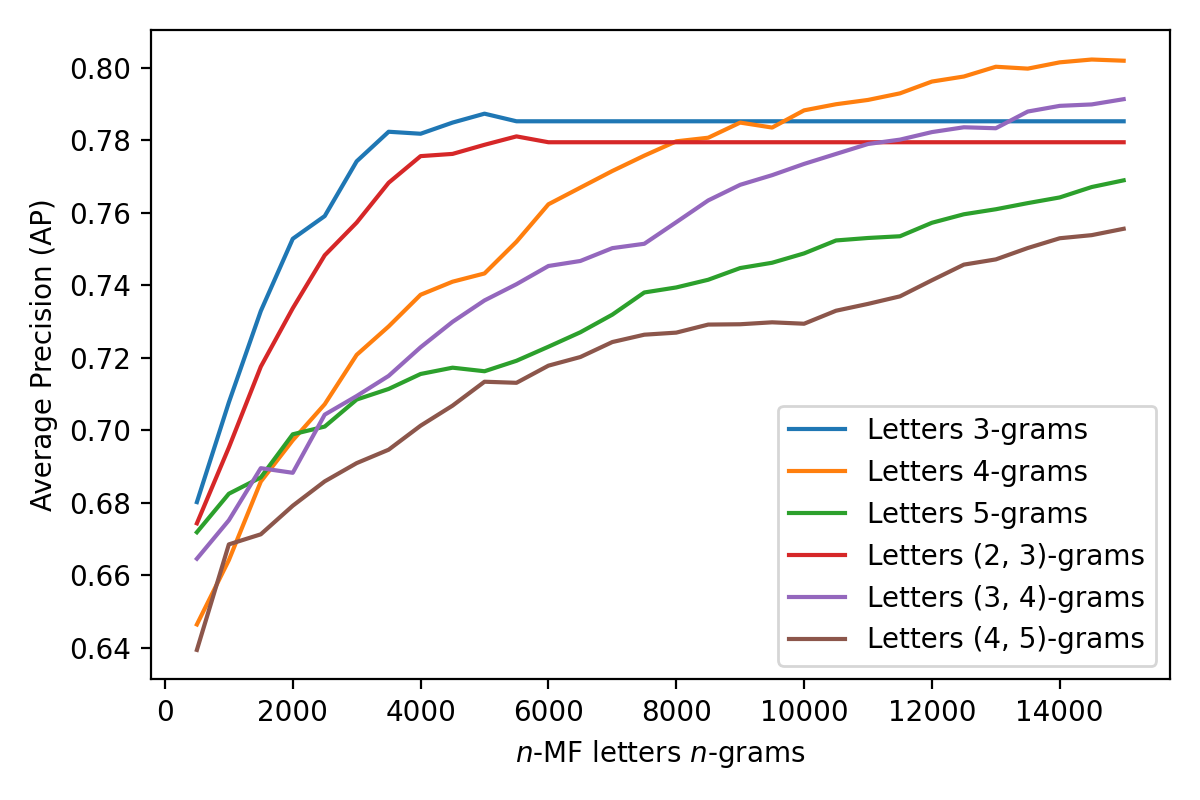
\includegraphics[width=\linewidth]{img/letter_ngrams_oxquarry.png}

  \vspace{0.5cm}

  \subcaption{Brunet}
  \label{fig:letter_ngrams_brunet}
  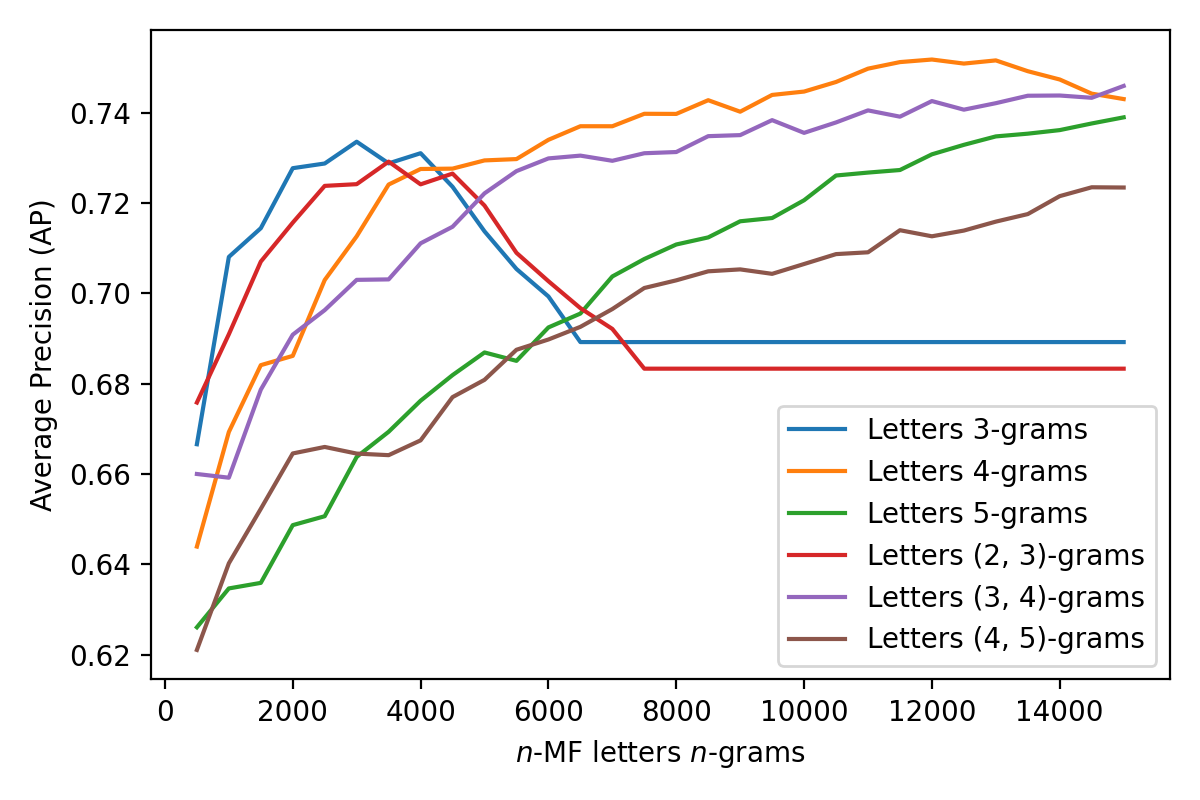
\includegraphics[width=\linewidth]{img/letter_ngrams_brunet.png}

  \vspace{0.5cm}

  \subcaption{St-Jean}
  \label{fig:letter_ngrams_st_jean}
  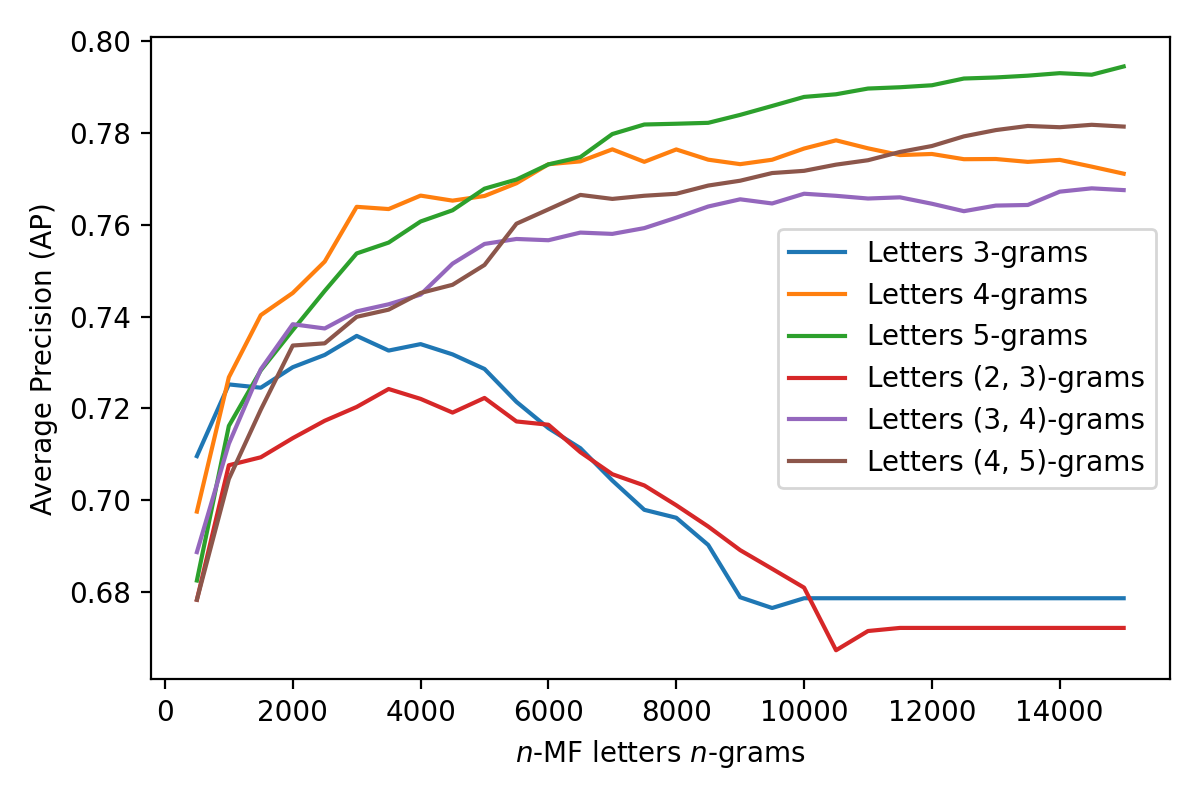
\includegraphics[width=\linewidth]{img/letter_ngrams_st_jean.png}
\end{figure}

\textbf{Second part}

As stated earlier, in the second part the objective it to compare the distance metrics with the $3$-grams/$3000$-MF and $4$-grams/$8000$-MF.
The distance metrics used are the ones presented in Section~\ref{sec:vectors_distances}.
The results for this experiment are in Table~\ref{tab:letter_ngrams}.
Since the number of MF and the size of the $n$-grams was optimized on the Cosine distance, the results may be biased.

For the $3$-grams, the following results can be observed:
The Cosine distance give the best results.
Though, two distances metrics can compete with the Cosine distance on certain datasets with the $3$-grams approach, namely the Manhattan distance and the Clark distance.
A worth noticing results, is the Euclidean distance, which have polarized results: on Oxquarry the average precision is $0.72$ and on St-Jean only $0.47$.
Using the right distance measure can have a relative increase up to $36$\%, when comparing the worse distance metric to the best of each dataset.

For the $4$-grams approach, as for the $3$-grams the Cosine is the best measure with this configuration.
The Manhattan distance and the Clark distance also are the second choice.
The Euclidean distance have the same behavior as for $3$-grams on the dataset.
For this configuration of $4$-grams with $8000$-MF, using the right distance measure is less impactful than the $3$-grams approach but still can have a relative increase in performance of $28$\% when changing from the worse distance metric to the best, with these datasets.

\begin{table}
  \centering
  \caption{Average precision for $n$-grams with every metrics, on the 3 datasets (best result for the dataset in bold).}
  \label{tab:letter_ngrams}

  \subcaption{$3$-grams with $3000$-MF}
  \begin{tabular}{l c c c}
    \toprule
    Distance metric & Oxquarry & Brunet & St-Jean \\
    \midrule
    Manhattan & \textbf{0.77} & 0.66 & 0.62 \\
    Tanimoto & 0.64 & 0.66 & 0.62 \\
    Euclidean & 0.72 & 0.63 & 0.47 \\
    Matusita & 0.60 & 0.66 & 0.58 \\
    Clark & 0.64 & \textbf{0.73} & 0.63 \\
    Cosine & \textbf{0.77} & \textbf{0.73} & \textbf{0.74} \\
    KLD & 0.57 & 0.65 & 0.54 \\
    JD & 0.58 & 0.66 & 0.56 \\
    \bottomrule
  \end{tabular}

  \vspace{0.5cm}

  \subcaption{$4$-grams with $8000$-MF}
  \begin{tabular}{l c c c}
    \toprule
    Distance metric & Oxquarry & Brunet & St-Jean \\
    \midrule
    Manhattan & 0.76 & 0.69 & 0.73 \\
    Tanimoto & 0.68 & 0.68 & 0.68 \\
    Euclidean & 0.73 & 0.65 & 0.55 \\
    Matusita & 0.63 & 0.68 & 0.65 \\
    Clark & 0.67 & 0.72 & 0.75 \\
    Cosine & \textbf{0.78} & \textbf{0.74} & \textbf{0.78} \\
    KLD & 0.61 & 0.66 & 0.60 \\
    JD & 0.61 & 0.67 & 0.63 \\
    \bottomrule
  \end{tabular}
\end{table}

\subsubsection{MF In-word $n$-grams / $n$-First / $n$-Last Evaluation}

In this experiment, the goal is to compare the three following substring text representations : In-word $n$-grams, $n$-First and $n$-Last.

Only the Z-Score normalized Cosine distance used and is evaluated using the average precision.
For this experiment, the number of $n$-MF variate between 200 and 4000 with a step of 100.
The $n$ for the In-word $n$-grams, $n$-First and $n$-Last variate between 3 and 5.

Figure~\ref{fig:first_last_letters_ngrams} shows the average precision for this experiment on the three datasets (Oxquarry, Brunet, St-Jean).

In the three dataset, the $3$-Last and $3$-First gives a lower average precision and quickly converge to an equilibrium value at around $1500$-MF.
For the three methods, when $n = 5$, it tends to produce better results than $n = 3$ or $n = 4$ as the $n$-MF increase.
In the Oxquarry corpus, in-word $4$-grams and in-word $5$-grams give an outstanding $\sim 95.0\%$ in average precision.
But this method is not as effective for the Brunet dataset.
For the Brunet dataset, the $5$-First can a good results compared to other text representations with small MF vector size.
And for St-Jean, the $5$-First with a small MF vector size give the best results.

No clear best configuration can be extracted with these results since the results are mixed across datasets, thus for this experiment, no text representation / distance measure are retained.

\begin{figure}
  \centering
  \caption{Average precision over the $n$-MF In-word $n$-grams, $n$-First and $n$-Last using Z-Score normalized Cosine distance}
  \label{fig:first_last_letters_ngrams}

  \subcaption{Oxquarry}
  \label{fig:first_last_letters_ngrams_oxquarry}
  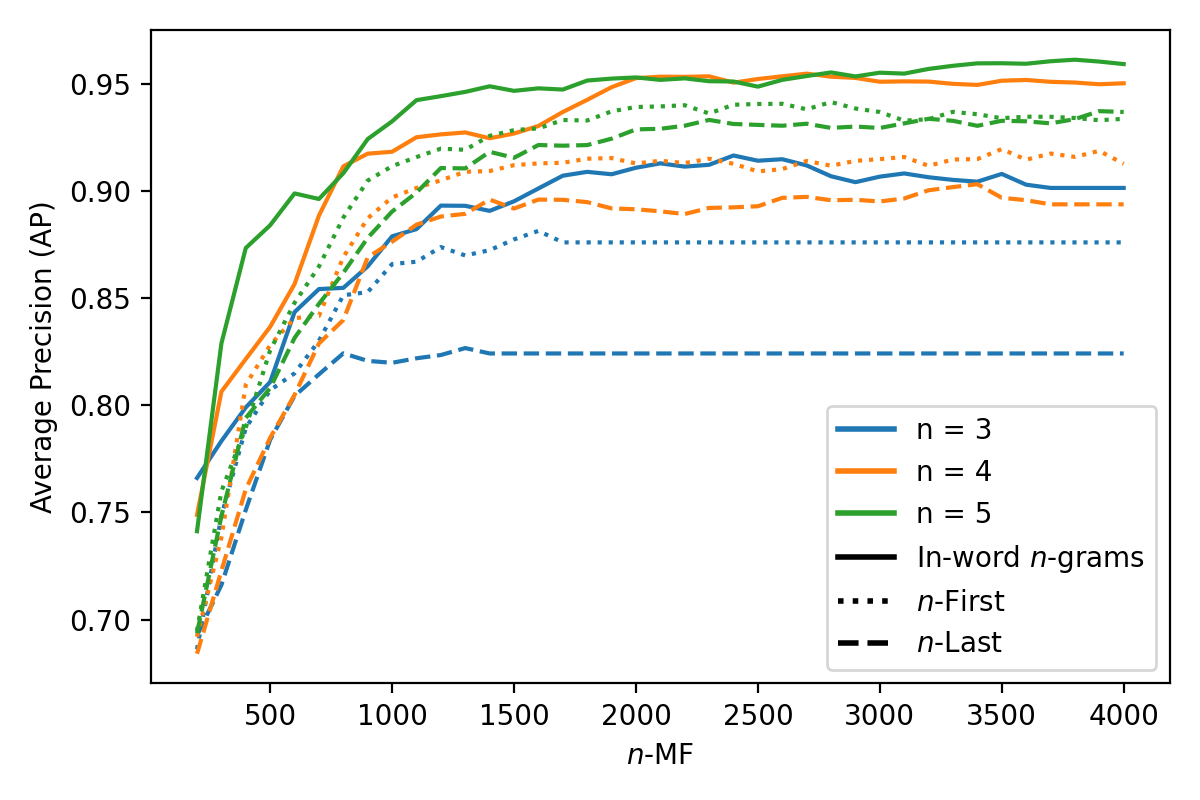
\includegraphics[width=\linewidth]{img/first_last_letters_ngrams_oxquarry.png}

  \vspace{0.5cm}

  \subcaption{Brunet}
  \label{fig:first_last_letters_ngrams_brunet}
  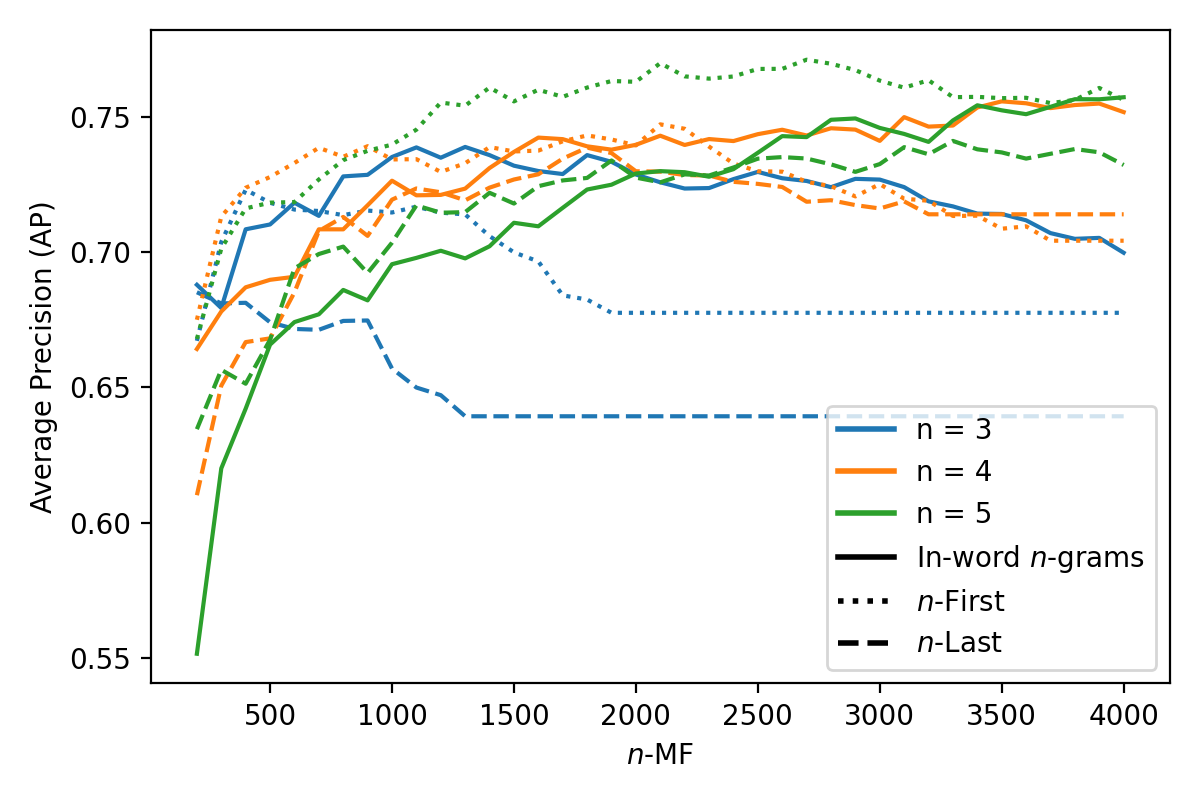
\includegraphics[width=\linewidth]{img/first_last_letters_ngrams_brunet.png}

  \vspace{0.5cm}

  \subcaption{St-Jean}
  \label{fig:first_last_letters_ngrams_st_jean}
  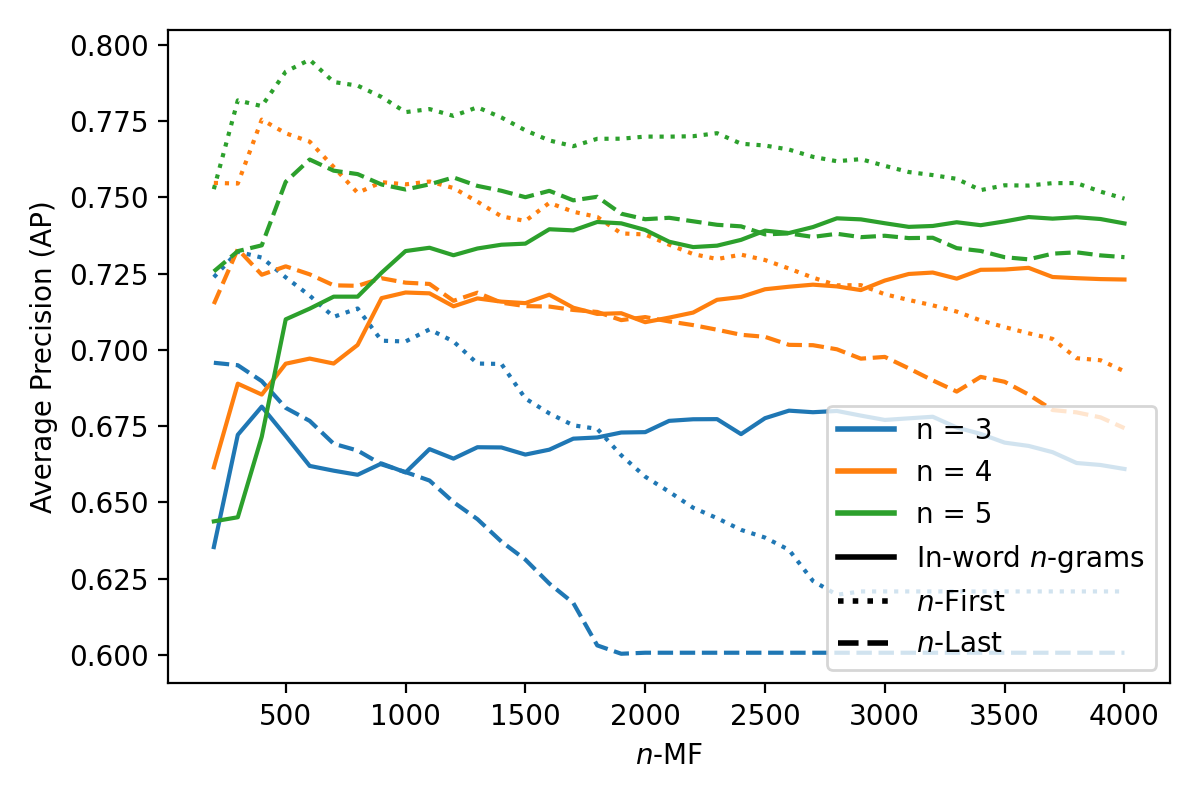
\includegraphics[width=\linewidth]{img/first_last_letters_ngrams_st_jean.png}
\end{figure}
